\documentclass{article}
\author{Toby {Cathcart Burn}}
\title{The Area of the Pythagoras Tree}

\usepackage{tikz}
%\usetikzlibrary{lindenmayersystems}
\usepackage{ifthen}
\usepackage{pgf}
\usepackage{wrapfig}
\usetikzlibrary{automata,positioning} 

\newcommand{\bounding}{
\draw[tsty] (-2.5,1) -- (-1.5,0) -- (2.5,0) -- (3.5,1) -- (3.5,2.5) -- (2,4) -- (-1,4) -- (-2.5, 2.5) -- cycle;
%\draw[tsty] (-3,1) -- (-2,0) -- (3,0) -- (4,1) -- (4,2) -- (2,4) -- (-1,4) -- (-3, 2) -- cycle;
}

\newcommand{\subt}[2]{
    \begin{scope}[yshift=1cm,rotate=45,scale=0.7071]
        #1
    \end{scope}
    \begin{scope}[xshift=0.5cm,yshift=1.5cm,rotate=-45,scale=0.7071]
        #2
    \end{scope}
}
\newcommand{\dup}[1]{\subt{#1}{#1}}
\newcommand{\tree}[1]{
    \fill[tsty] (0,0) -- (1,0) -- (1,1) -- (0,1) -- cycle;
    \ifthenelse{#1<2}{}{
        \dup{\tree{\the\numexpr#1-1}}
    }
}
\newcommand{\outertree}[1]{
    \fill[tsty] (0,0) -- (1,0) -- (1,1) -- (0,1) -- cycle;
    \ifthenelse{#1<2}{
        \bounding
    }{
        \dup{\outertree{\the\numexpr#1-1}}
    }
}
\newcommand{\depth}{5}%Means that rendering doesn't take so long while 
\begin{document}
\maketitle
\begin{abstract}
The area of the Pythagoras Tree is exactly
    
${12823413011547414368862997525616691741041579688920794331363953564934456759066858494476606822552437442098640979}\over{877512406035620068631903180662851572553488753575243048137500508983979170248733422547196905684808937723408093}$.
    
This can be shown by describing the Pythagoras Tree using a non-deterministic Buchi automaton with 103 states %(28-3)*4-2+1+4
and a 4 symbol alphabet.
\end{abstract}
\section{Introduction}\label{sec:intro}
The Pythagoras Tree is a fractal constructed by taking a unit square and then recursively constructing 2 copies of the Pythagoras tree each scaled by a factor of $1/\sqrt{2}$ and rotated $45^\circ$ so that the bases of the copies of the original square form a right-angled isosceles triangle with the top edge of the original square.

\begin{center}
    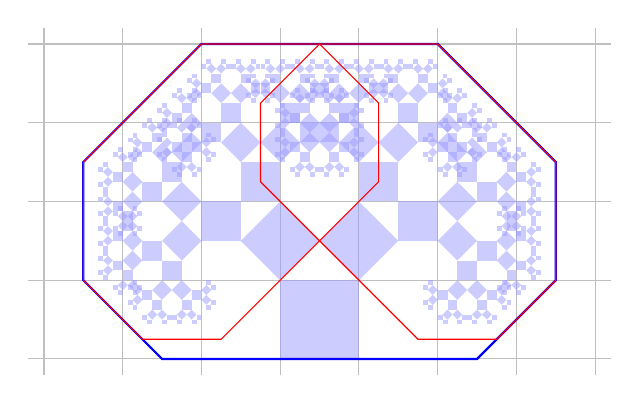
\begin{tikzpicture}[scale=1]
\draw[color=lightgray, step=1] (-3.2,-0.2) grid (4.2,4.2);
    \tikzstyle{tsty}=[fill=blue!40,opacity=0.5]
\tree{9}
\tikzstyle{tsty}=[color=blue,thick]
\bounding
\tikzstyle{tsty}=[color=red]
\dup{
    \bounding
}
\end{tikzpicture}
\end{center}
\newpage
\section{Defintions}
\subsection{Area}
\begin{wrapfigure}{l}{1.5cm}
\centering
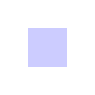
\begin{tikzpicture}[scale=0.5]
    \tikzstyle{tsty}=[fill=blue!40,opacity=0.5]
    \tree{1}
\end{tikzpicture}

Depth 1

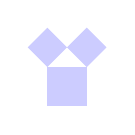
\begin{tikzpicture}[scale=0.5]
    \tikzstyle{tsty}=[fill=blue!40,opacity=0.5]
    \tree{2}
\end{tikzpicture}

Depth 2

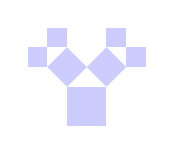
\begin{tikzpicture}[scale=0.5]
    \tikzstyle{tsty}=[fill=blue!40,opacity=0.5]
    \tree{3}
\end{tikzpicture}

Depth 3

\end{wrapfigure}

We define the \emph{depth 1 rendering} of the Pythagoras tree to consist of a unit square, and the depth $n+1$ rendering to consist of 2 transformed copies of the depth $n$ rendering together with the open unit square, arranged as described in Sec. \ref{sec:intro}. The Pythagoras tree is the union of the sequence of finite depth renderings.


This paper sets out to find the exact area of the Pythagoras tree, which we will denote $A$. $A$ is the limit of the sequence of the areas for each tree rendered to a specific depth.
This sequence starts $1,2,3,4,5,5 {15\over 16},6 {53\over 64},\cdots$. The limit of this monotone sequence exists since it is bounded above by the area of a $7 \times 4$ rectangle which no part of the shape leaves.

Whether the squares are open or closed has no effect on the area of finite depth rendering, therefore has no effect on the limit of the sequence of areas. Since the Pythagoras tree is not closed, even if closed squares are used rather than open ones, 
Whether the closure of the limit of the sequence has a different area from the limit of the sequence is a different question that could be addressed directly, but will be shown to be false in the process of finding the area. 

\subsection{Automata}

\begin{wrapfigure}{l}{2.1cm}
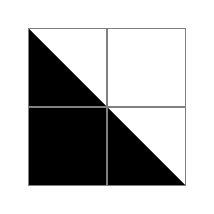
\begin{tikzpicture}
\fill (0,0) -- (2,0) -- (0,2) -- cycle;
\draw[gray] (0,0) grid (2,2);
\end{tikzpicture}
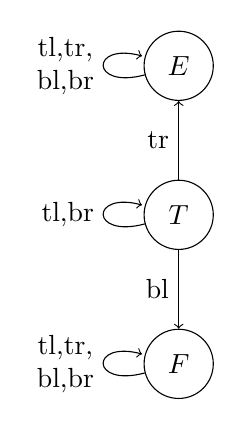
\begin{tikzpicture}[auto]
\node[state] (t) {$T$};
\node[state] (e) [above=of t] {$E$};
\node[state] (f) [below=of t] {$F$};
\path[->]
(t) edge node[swap] {bl} (f)
    edge node {tr} (e)
    edge [loop left] node {tl,br} ()
(e) edge [loop left] node[align=center] {tl,tr,\\bl,br} ()
(f) edge [loop left] node[align=center] {tl,tr,\\bl,br} ();
\end{tikzpicture}
\end{wrapfigure}

Certain subsets of a unit square can be represented by dividing the square into 4 corners and describing what each looks like. For shapes in which parts are copies of the whole, this can be done using a finite state automaton with the alphabet consisting of 4 symbols: tl (top left), tr (top right), bl (bottom left) and br (bottom right). For example, the triangle shown to the left can be described by the automaton below it. The top left and bottom right corners are smaller copies of the triangle, while the bottom left and top right corners are full and empty respectively.

This representation lets us calculate the area of the triangle. Call the area of the triangle $A_T$. Since the area of the triangle is the sum of the areas of each of the 4 corners, we have that $A_T = A_F/4 + 2A_T/4 + A_E/4$ where $A_F$ is the area of a full square and $A_E$ is the area of an empty square. As $A_F=1$ and $A_E=0$, we the equation becomes $A_T = 1/4 + A_T/2$. This lets us conclude that $A_T = 1/2$ i.e. the area of the triangle is exactly half that of the unit square.

%technically we're using ω-automata, which accept or reject infinte strings (F is the only accepting state, and every path that reaches it stays there forever, so we don't need a very fancy acceptance condition).
%some points have multiple representations as infinite strings, but almost all of them don't, so we don't need to worry about them when calculating the area.
%Every open subset of the unit square can be described in this manner, if infinitely many states are allowed.
\ 

\ 

 
 \newpage
\subsection{Non-deterministic Automata}
Overlapping shapes can be described by non-deterministic automata where each node may have multiple (or zero) edges with a given label. In this case we don't need a separate state for empty squares - if a corner of a node is empty, it may simply have no outgoing edges with that label.

For our purposes, any given non-deterministic automaton may be converted to a deterministic automaton by having a node in the new one for every set of nodes in the old one. The node corresponding to the set $S$ should have an edge labeled $l$ to set of all nodes in the old automaton with edges labeled $l$ from some element of $S$, and all sets containing the full node $F$ may be collapsed into one, with edges to itself.


\section{Describing the Pythagoras tree using an automaton}
One way to look at the Pythagoras tree is as 4 copies of itself, together with the 3 squares in the depth 2 rendering.
\begin{center}
	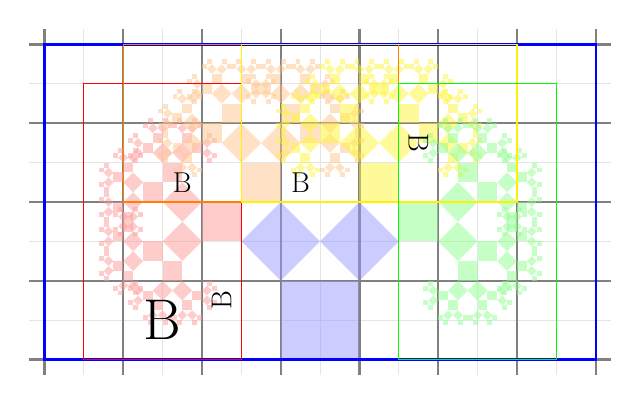
\begin{tikzpicture}[scale=1]
		\draw[color=lightgray!40, step=0.5] (-3.2,-0.2) grid (4.2,4.2);
		\draw[color=gray,thick, step=1] (-3.2,-0.2) grid (4.2,4.2);
		\draw[color=red] (-3,0) rectangle (4,4);
		\tikzstyle{tsty}=[fill=blue!40,opacity=0.5]
		\tree{2}
		\subt{\subt{
				\tikzstyle{tsty}=[fill=red!40,opacity=0.5]
				\tree{7}
			}{
				\tikzstyle{tsty}=[fill=orange!45,opacity=0.5]
				\tree{7}
		}}{\subt{
				\tikzstyle{tsty}=[fill=yellow!80,opacity=0.5]
				\tree{7}
			}{
				\tikzstyle{tsty}=[fill=green!45,opacity=0.5]
				\tree{7}
			}}
		
%		\dup{\dup{
%				\tree{7}
%		}}
		\draw[color=blue,thick] (-3,0) rectangle (4,4);
		\tikzstyle{tsty}=[color=red]
		\subt{\subt{
				\draw[color=red](-3,0) rectangle (4,4);
			}{
				\draw[color=orange](-3,0) rectangle (4,4);
		}}{\subt{
				\draw[color=yellow](-3,0) rectangle (4,4);
			}{
				\draw[color=green](-3,0) rectangle (4,4);
		}}
	\path (-1.5,0.5) node[node font=\huge] {B};
	\dup{\dup{	\path (-1.5,0.5) node [transform shape,node font=\huge] {B};}}
%		\dup{\dup{
%			\draw[color=red] (-3,0) rectangle (4,4);
%		}}
	\end{tikzpicture}
\end{center}
The tree may be divided into 28 squares in a $7\times4$ grid so that the largest square in the tree exactly fills one square of the grid. The 4 copies described above are nicely aligned to a subdivision of the grid, allowing each square of the grid to be described as it 4 corners, each of which is either full, empty, a triangle, or an overlapping combination of squares of the original grid and their rotations. This lets us construct a non-deterministic automaton describing the shape.

As all rotations are multiples of $90^\circ$, there are only 4 states needed for each of the 28 original cells. the transitions from rotations are straightforward given the transitions from the originals. This gives a nondeterministic automaton with $4\times28+4+1 = 117$ states (the initial 28, their rotations, 4 triangles and 1 full square). This can be transformed into a deterministic automaton with $2^{116}+1$ states, but fortunately not all of them are needed. Instead we can start from the 28 singleton sets representing squares of the grid and discover that ${\sim}10000$ states are reachable from those, which can be reduced to ${\sim}1000$ by accounting for rotations and reflections.

This gives a system of linear equations for the area of the shape described by each state. This system of equations has exactly one solution.

Noting that the area of the closure of the Pythagoras tree would also be a solution to that system of linear equations, the fact that it has a unique solution implies that taking the closure does not change the area.

\section{Further results}
We can also use this method to find the area of the Pythagoras tree with the internal triangles filled in, and to calculate the area of the C-dragon.

\appendix
\section{State machine}
\section{System of Linear equations}
\section{Code}


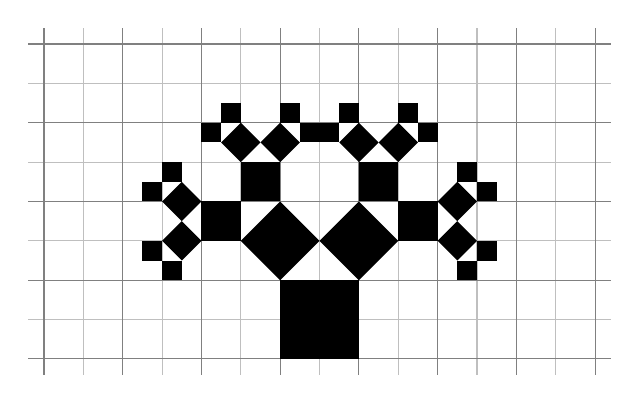
\begin{tikzpicture}[scale=1]
    \draw[color=lightgray, step=0.5] (-3.2,-0.2) grid (4.2,4.2);
    \draw[color=gray, step=1] (-3.2,-0.2) grid (4.2,4.2);
    \tikzstyle{tsty}=[]
    \tree{\depth}
\end{tikzpicture}

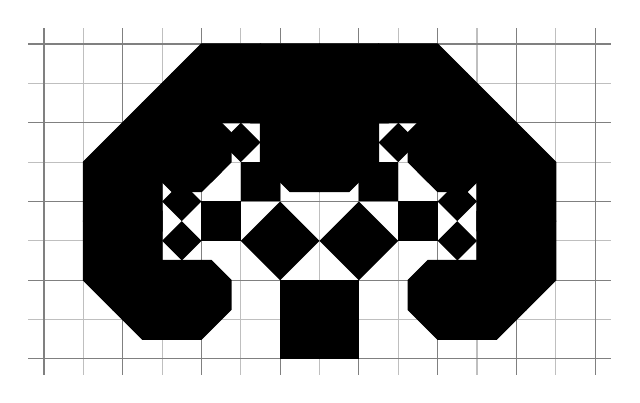
\begin{tikzpicture}[scale=1]
    \draw[color=lightgray, step=0.5] (-3.2,-0.2) grid (4.2,4.2);
    \draw[color=gray, step=1] (-3.2,-0.2) grid (4.2,4.2);
    \tikzstyle{tsty}=[fill=black]
    \outertree{\depth}
\end{tikzpicture}

\end{document}
